\section{Project}
\labelsec{Project}
%===========================================================================
\subsection{Database e Altre Rappresentazioni di Dati}

Per la gestione del database si \`e scelto di utilizzare un database NoSql, nell'accezione MongoDB\cite{MongoDB}. In questa sede non si discuteranno i vantaggi, gli svantaggi o le particolarit\`a di questa tecnologia in quanto \`e stato fatto gi\`a ampiamente durante il corso. Di seguito si riportano gli schemi dei documenti che sono stati salvati, le collezioni e il significato di alcuni dei valori inseriti.

\begin{center}
\textbf{Collection Ranges}
\end{center}

In questa collezione di documenti vengono raggruppati tutti i documenti relativi ai ranges che sono da controllare. In particolare sono stati individuati due tipologie di range in base alla tipologia di sensori.

\begin{itemize}
  \item Si/No: Per quella tipologia di sensori che non forniscono effettivamente dei valori ma che notificano solamente la presenza o l'assenza di un particolare elemento come il GAS o il movimento.
  \item  Valore: validi quando un sensore effettivamente serve una misurazione di una grandezza, come ad esempio la temperatura. In questo caso \`e utile sapere se questa grandezza rimane all'interno di determinati range.
\end{itemize}

\begin{figure}[ht]
\centering
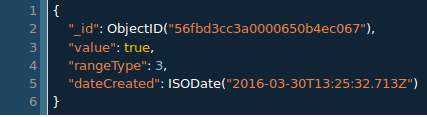
\includegraphics[width=\textwidth,natwidth=610,natheight=642]{Figures/DataStructures/RangesBoolean.png}
\caption{Documento dei Ranges Booleani}
\end{figure}

\begin{figure}[ht]
\centering
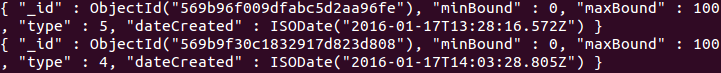
\includegraphics[width=\textwidth,natwidth=610,natheight=642]{Figures/DataStructures/RangesValues.png}
\caption{Documento dei Ranges di Valori}
\end{figure}

Si vuole far notare come sia comunque sempre presente un attributo di tipo data in modo da poter filtrare i range in base al tempo di inserimento e la presenza di un valore numerico che in questo caso rappresenta il tipo di range.

Per indicare il tipo di range si riporta il listato scala che indica tale tipologia.

\begin{figure}[ht]
\centering
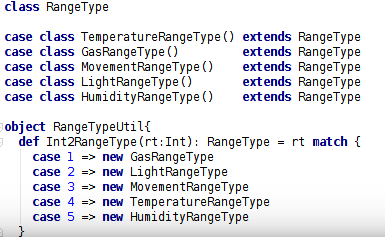
\includegraphics[scale=0.5,natwidth=610,natheight=642]{Figures/DataStructures/Ranges.png}
\caption{Valore Numerico dei Ranges}
\end{figure}

\begin{center}
  \textbf{Collertion Sensors}
\end{center}

Per quanto riguarda la collezione dei sensori si utilizza un'apposita collection. Questa non sar\`a modificata spesso, e serve principalmente per eventuali evoluzioni del progetto, in modo che sia gi\`a presente. Anch'essi sono dotati di di tipo come i range e, per questa implementazione, i tipi coincidono. A livello di progetto per\`o si \`e deciso di mantenerli separati nel caso in un futuro questi divergano. Inseriamo di seguito un'immagine che rappresenta come \`e strutturato un documento di un sensore.

\begin{figure}[ht]
\centering
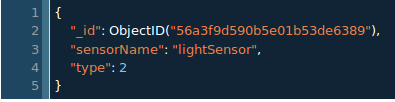
\includegraphics[scale=0.5,natwidth=610,natheight=642]{Figures/DataStructures/SensorsValues.png}
\caption{Rappresentazione a DB dei Sensori}
\end{figure}


\begin{figure}[ht]
\centering
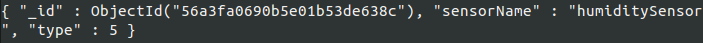
\includegraphics[scale=0.5,natwidth=610,natheight=642]{Figures/DataStructures/Sensors.png}
\caption{Valore Numerico dei Sensori}
\end{figure}

\afterpage{\clearpage}

\newpage

\begin{center}
\textbf{Collection Data}
\end{center}

Per quanto riguarda la rappresentazione dei dati raccolti, anche in questo caso sono presenti 2 tipologie di dati, che a loro volta differiscono leggermente per la tipologia di dato, se booleano o meno:
\begin{itemize}
\item Dati Corretti: cio\`e quella tipologia di dati che rientrano all'interno del range prestabilito per la loro tipologia.
\item Dati Incorretti: quelli che invece non rientrano nella tipologia corretta e quindi vanno a violare il range attivo.
\end{itemize}

Come si pu\`o osservare il primo tipo \`e pi\`u semplice in quanto non richiede di salvare anche l'informazione riguardante di quanto il dato risulta errato. Di seguito come fatto in precedenza si indica un esempio di struttura di un dato corretto e non corretto per ogni tipologia di dato.

\begin{figure}[ht]
\centering
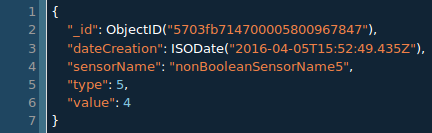
\includegraphics[scale=0.5,natwidth=610,natheight=642]{Figures/DataStructures/DataNoViolation.png}
\caption{Dato Non Booleano Corretto salvato in database}
\end{figure}

Come si pu\`o osservare non \`e stato comunque inserito un valore per la violazione in modo da poter distinguere meglio i dati violati da quelli invece corretti.

\begin{figure}[ht]
\centering
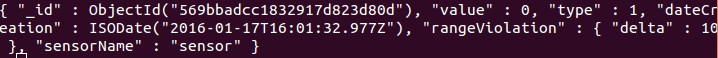
\includegraphics[scale=0.5,natwidth=610,natheight=642]{Figures/DataStructures/DataViolation.png}
\caption{Dato Non Booleano Non Corretto salvato in database}
\end{figure}

In questo caso appunto il valore della violazione non e' piu' nullo ma contiene un semplice campo \textit{delta} che indicher\`a la differenza rispetto al range. In particolare questo sar\`a positivo se il valore registrato supera il range attuale, negativo se invece \`e troppo basso o zero se il tipo di sensoristica e quindi anche di range \`e booleano. Come si puo' vedere nelle seguenti immagini.

\begin{figure}[ht]
\centering
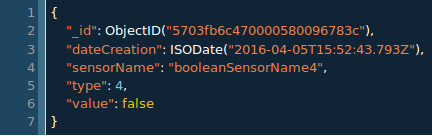
\includegraphics[scale=0.5,natwidth=610,natheight=642]{Figures/DataStructures/BooleanDataNoViolation.png}
\caption{Dato Booleano Corretto salvato in database}
\end{figure}

\begin{figure}[ht]
\centering
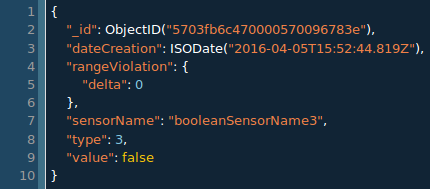
\includegraphics[scale=0.5,natwidth=610,natheight=642]{Figures/DataStructures/BooleanDataViolation.png}
\caption{Dato Non Booleano Non Corretto salvato in database}
\end{figure}

\afterpage{\clearpage}

\newpage

\begin{center}
  \textbf{Rappresentazione Dati Attraverso la Rete}
\end{center}

Oltre alla rappresentazione dei dati per quanto riguarda i dati salvati all'interno del Database \`e stato necessario concordare una rappresentazione di dati che verranno inviati attraverso la rete. Non necessariamente le due rappresentazioni devono coincidere in quanto, i dispositivi dai quali si ricavano i dati posso avere diversi formati e modalit\`a di ottenere tali valori, quindi di conseguenza questa rappresentazione \`e sbilanciata rispetto a chi invia i dati, cio\`e il sistema embedded.

Anche per la rappresentazione dei dati si \`e scelta la rappresentazione JSON in quanto questa \`e una delle pi\`u utilizzate nella comunicazione eterogenea via rete, si pone quindi come formato interoperabile tra varie tecnologie, come accade nel nostro caso.

Di seguito si riporta un esempio di dati in formato JSON:

\begin{lstlisting}[language=json]
  {
    "sensorName": "nomeSensore",
    "sensorType": 1,
    "value": true,
    "date": "2016-04-05 17:52:55.058"
  }
\end{lstlisting}

Si veda il tipo di sensore dai valori indicati precedentemente e si sottolinea che il tipo del campo \textit{value} pu\`o essere sia booleano che numerico.

\subsection{Introduzione All'Architettura di Progetto}

Nelle prossime sezioni si vuole inserire le modifiche che sono state fatte alla architettura logica appena introdotta, ma cercando di evitare di ripetere aspetti che non sono effettivamnete cambiati. Di conseguenza si \`e deciso di riportare solamente quegli aspetti che sono stati modificati in base alle scelte tecnologiche effettivamente fatte.\\
In ogni caso si \`e deciso di cercare il pi\`u possibile di sfruttare quanto gi\`a \`e stato concordato dagli analisti cercando di effettuare meno modifiche possibili all'architettura, ma allo stesso tempo di cercare di ridurre le entit\`a che, per ragioni tecnologiche, risultano inutili per la creazione del progetto.

\begin{center}
  \textbf{Server}
\end{center}

\subsection{Struttura}

Vista l'introduzione della tecnologia in questa fase si \`e deciso di apportare alcune modifiche architetturali. Si riporta una lista di modifiche apportate all'architettura:

\begin{itemize}
  \item \textit{DataStructures:} Si \`e ritenuto necessario introdurre un'ulteriore package che non era stato previsto precedentemente contenente le rappresentazioni interne in forma di classi dei dati che circolano nel sistema, cos\`i come delle classi di utilit\`a che servono per la conversione, da e verso, questi dati. (eg . JSON, BSON, DATETIME)
  \item \textit{IDataFormatter:} Visto che le elaborazioni di trasformazione dei dati non richiedono tanta computazione si \`e deciso di eliminare il metodo che, dato un valore lo validava inglobandolo direttamente dentro il primo metodo che restituisce lo stream. Inoltre nella costruzione dello stream ci si \`e accorti che il valore dell'input non viene passato per parametro al metodo, ma viene gestito dall'infrastruttura, quindi si \`e deciso di eliminarlo. Spesso gli oggetti che validano e formattano i dati passano da una rappresentazione ad un'altra: tra valori JSON, BSON e classi interne per i dati.
  \item \textit{IDBDataFormatter:} Viene aggiunto un'ulteriore metodo che gestisce la creazione di dati da un formato inerente alle strutture dati presenti in un altro utilizzabile per lo storage dei dati nel DB. Questo metodo \`e estraneo a quelli per la costruzione di stream e serve per la gestione delle richieste di inserimento di un nuovo range.
  \item \textit{Eliminazione della Maggior Parte dei Formatter:} Questa scelta \`e data dalla possibilit\`a che PlayFramework e altre build in librerie che abbiamo utilizzato consentono per la conversione automatica dei dati da un formato ad un altro, di coseguenza queste operazioni vengono agilmente svolte all'interno del package DataStructures.
  \item \textit{Eliminazione del Presentator:} Anche in questo caso le funzionalit\`a di playframework ci hanno evitato questa implementazione.
  \item \textit{Eliminazione delle Factory:} Visto che la maggior parte delle classi che erano state pensate non inglobano uno stato, ma vengono utilizzate semplicemente per applicare delle computazioni allo stream allora sono state eliminate la maggior parte delle factory class. Grazie anche alla tecnologia scelta (scala) molte delle classi sono state convertite in objects (build-in singletons).
  \item \textit{Eliminazione della classe Configurator:} Si \`e deciso di eliminare tale classe in quando non \`e pi\`u possibile pensare a un entry point per l'applicazione, ma questa viene risvegliata attraverso chiamate rest e di conseguenza molti dei processi legati alla creazione di oggetti \`e stata ridotta.
  \item \textit{Eliminazione del Data Analysis:} A fronte delle semplici operazioni di analisi sui dati (Min, Max, Average) si \`e deciso di sfruttare direttamente le capacit\`a forniteci dal database.
  \item \textit{StreamBuilder:} Le classi che implementano gli stream builder sono state leggermente modificate. In particolare si \`e previsto uno stream builder per la creazione dello stream riguardante i dati, uno per il salvataggio dei dati e uno per la gestione dei range. Si vedano poi lo schema della struttura e interazione.
\end{itemize}

Si di seguito riporta quindi lo schema della struttura di progetto. Purtroppo per\`o alcune delle astrazioni presenti nel linguaggio scala non possono essere completamente catturate dal linguaggio di modellazione UML. Per rendere poi lo schema pi\`u pulito si \`e deciso di omettere tutte le implementazioni che non aggiungono valore alle interfaccie.

\begin{sidewaysfigure}[ht]
\centering
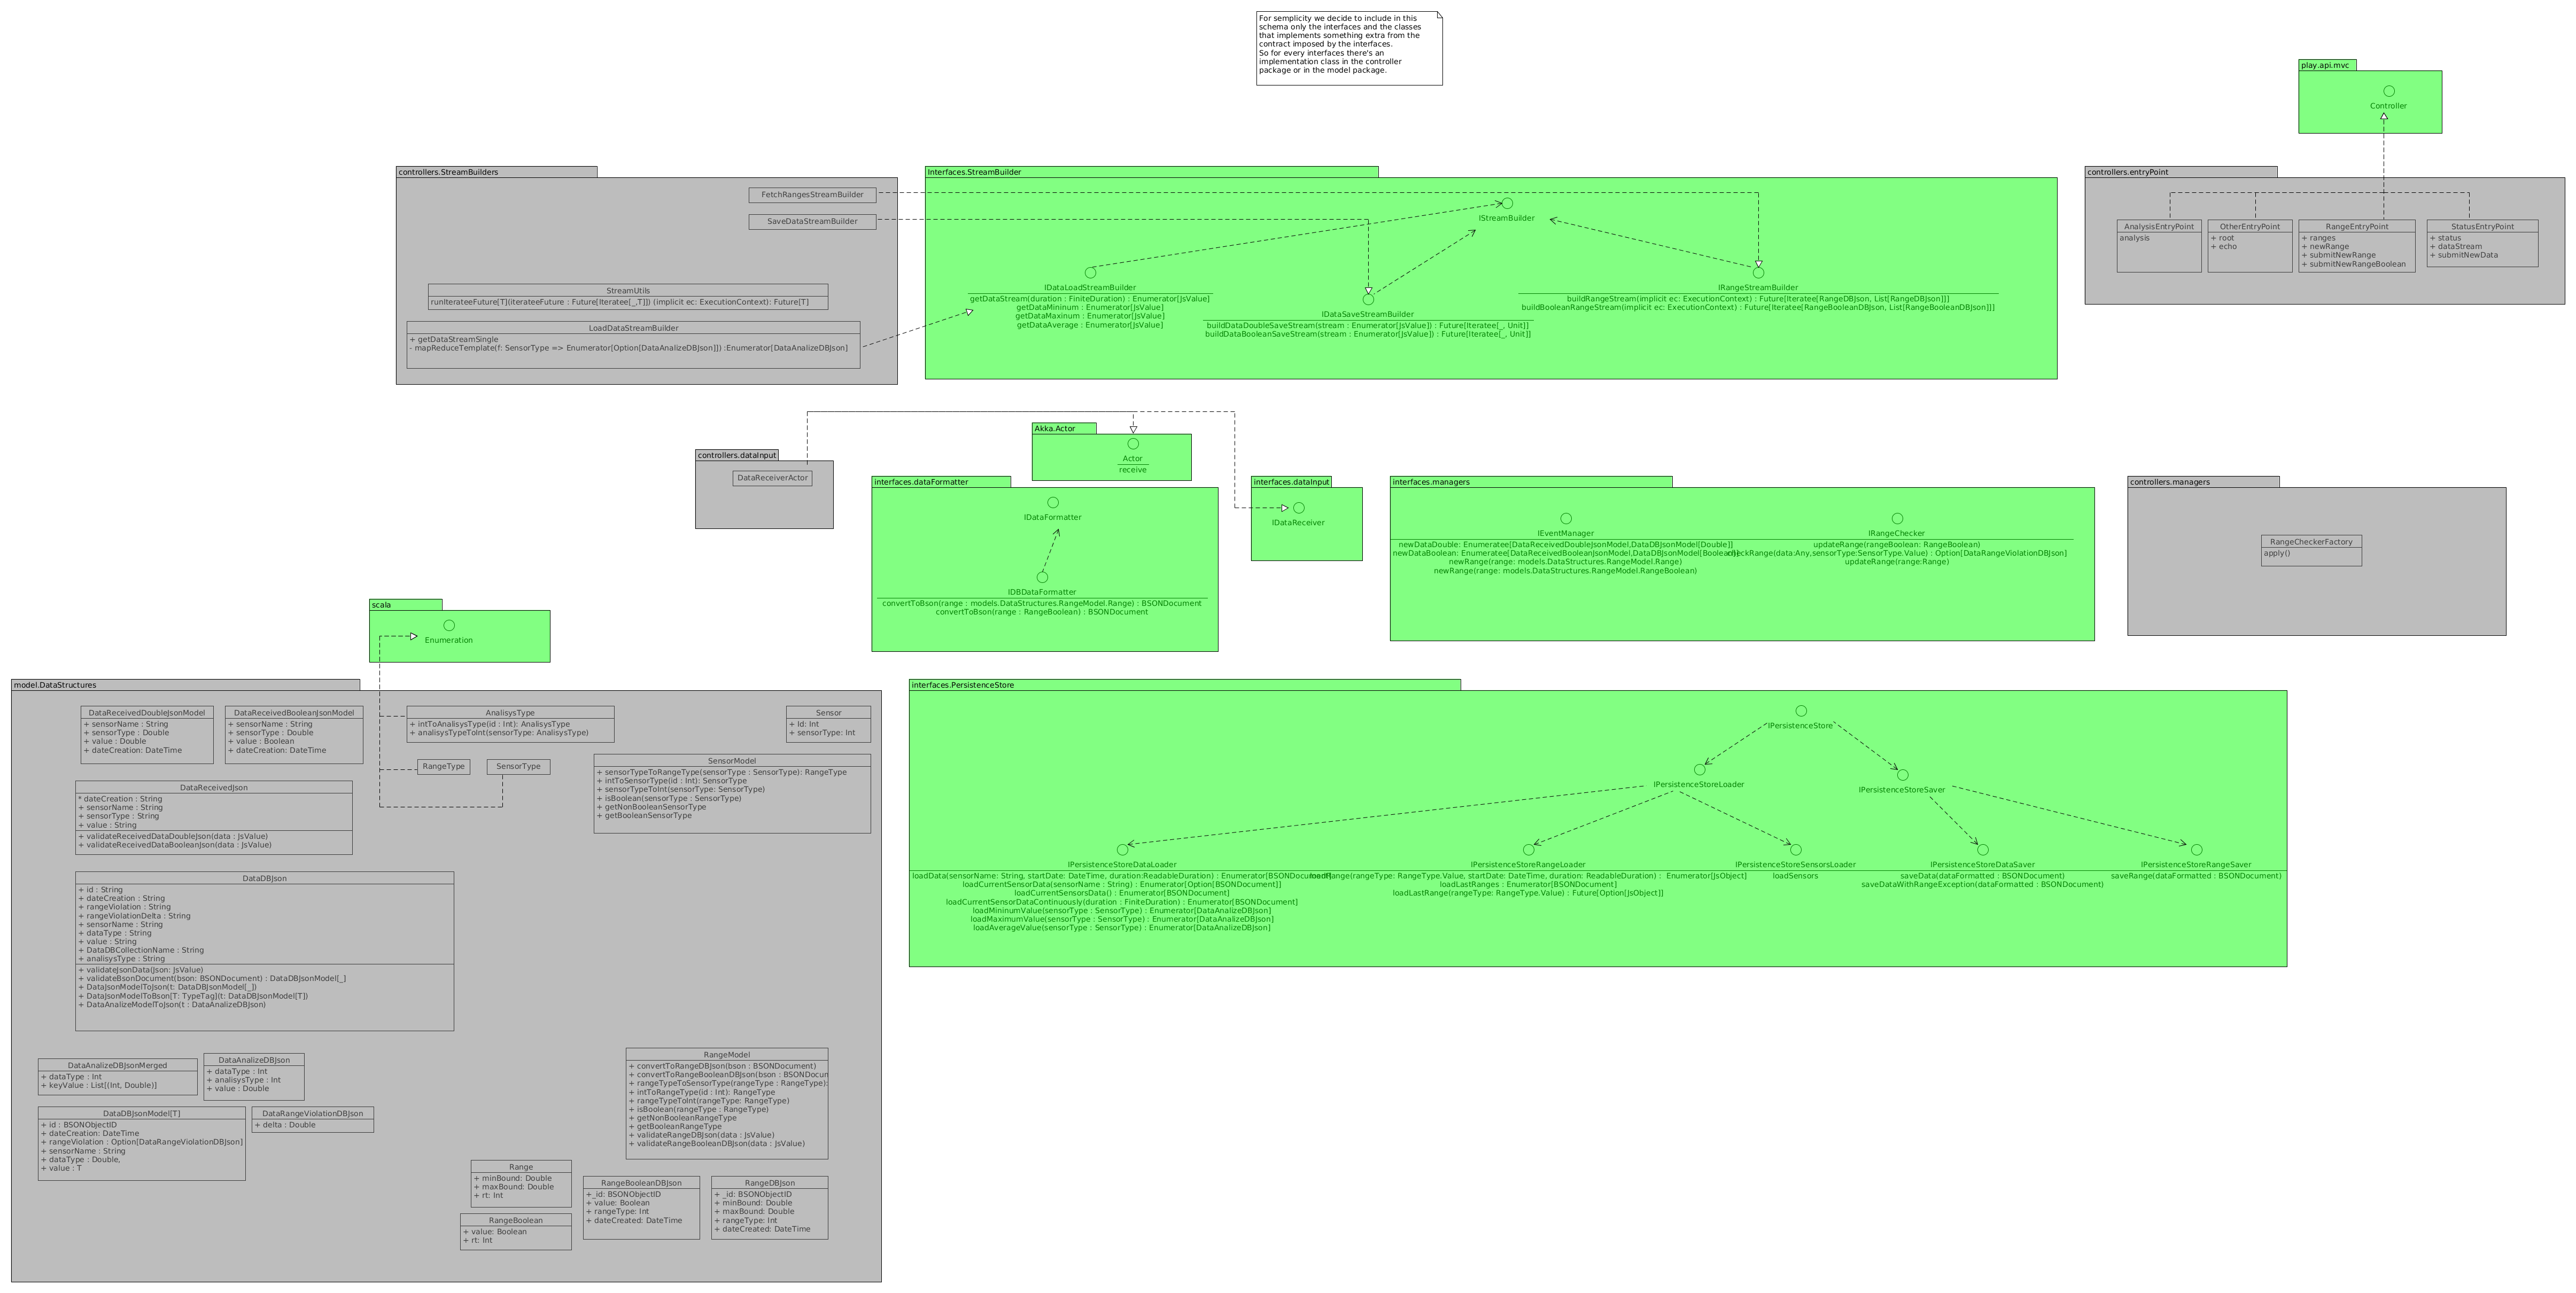
\includegraphics[scale=0.1]{Figures/Project/Server/Structure/DomoticRoomServerClassDiagram}
\caption{Struttura di progetto del Server}
\end{sidewaysfigure}

\afterpage{\clearpage}

\newpage

\subsection{Interazione}

In questa parte si riporta la tecnologia che si \`e utilizzata per effettuare l'interazione che si \`e analizzata e indicata in fase di analisi, lo stream. In particolare si \`e notato che, il framework play\cite{PlayFramework} gi\`a gestisce attraverso delle sue strutture la possibilit\`a di operare attraverso stream di dati. Questa possibilit\`a \`e stata introdotta dal framework per gestire meglio dati parziali o casi che richiederebbero molto tempo, come ad esempio un'upload di file cospiquo. Quindi ci avvarremo di questa astrazione per implementare quanto descritto nella fase di analisi del problema. Si riporta in bibliografia quindi la documentazione del framework che spiega il funzionamento di \textit{Enumerators,Iteratees e Enumeratees.} \cite{PlayStreaming}

Un'ulteriore modifica che va apportata visto che ci si trova in ambito web e si dispone di questo framework \`e la necessit\`a di eliminare o aggiungere alcune entit\`a previste precedentemente perch\'e, in fase realizzativa sono risultate ridondanti, ad esempio:
\begin{itemize}
\item \textbf{DataInputs:} Viene rimpiazzato dai controller che gestiscono direttamente le richieste POST al sistema per la gestione dei dati provenienti dai form HTTP, o dal sistema embedded. Saranno questi componenti, come ad esempio il \textit{RangeEntryPoint} a validare direttamente i dati in arrivo e a chiamare poi gli elementi successivi nel flusso di dati per il salvataggio di un nuovo range. Si veda l'analisi del problema.
  \item \textbf{DataReceiverActor: } Attore basato sul framework akka che consente di gestire lo stream di input, in particolare consente di aggiungere incrementalmente dati all stream mano a mano che questi arrivano senza che sia necessario ricrearlo.
\end{itemize}

Infine, visto che ci si trova in fase di progetto e che gli schemi principali sono gi\`a stati inseriti in fase di analisi, in questo punto si \`e deciso di inserire degli snippet di codice come schema di interazione in quanto, essendo provenienti dalla programmazione reactive risultano molto dichiarativi e quindi espressivi al fine della modellazione.

\paragraph{Stream di Salvataggio Dati:} di seguito vengono inseriti gli snippet principali che mostrano il salvataggio dei dati attraverso la costruzione e l'esecuzione di uno stream, in particolare nella prima (fig.\ref{SaveDataStream1}) si pu\`o osservare come i dati, provenienti dalla rete vengono controllati inizialmente se sono conformi alla specifica JSON e poi passati all'attore (fig.\ref{SaveDataStream2}) che costruisce uno stream con un canale incui possono essere inseriti a mano a mano nuovi dati. Infine nell'ultima parte si costruisce effettivamente tutto lo stream attraverso vari steps che consentono di salvare tali dati e controllarne la correttezza. (fig.\ref{SaveDataStream3})

\paragraph{Stream di Caricamento Dati:} Anche questo stream parte chiaramente dal controller in quanto, alla chiamata della pagina di stato dei sensori, viene prima richiesti i dati per il valore dei range (si veda il paragrafo apposito) i quali vengono passati alla vista che li user\`a per la visualizzazione dei limiti imposti da questi all'interno dei grafici. Successivamente sempre la vista richieder\`a i dati ad un tempo prefissato, in modo da comandare il flusso e evitare backpressure, attraverso l'utilizzo di una websocket instaurata tra client e server (fig \ref{LoadDataStream1}). Infine sempre lo streambuilder si occuper\`a di ottenere i dati attraverso una catena di computazioni come si pu\`o vedere in figura \ref{LoadDataStream2}

\paragraph{Stream di Caricamento Ranges:} Per quanto riguarda il caricamento dei ranges, utilizzato anche in figura \ref{LoadDataStream1} e nella relativa pagina di visualizzazione dei sensori, si utilizza uno stream che recupera i dati a database attraverso una query di raggruppamento che ottiene solamente i valori pi\`u aggiornati. In particolare gli stream sono due distinti sulla base della tipologia dei range in quanto, un tipo mostra i dati all'interno di valori numerici, mentre l'altro si occupa dei valori booleani, si veda la figura \ref{LoadRangeStream}

\paragraph{Stream di Caricamento Dati Analisi:} Anche per il recupero dei dati di analisi si utilizza l'astrazione a stream come si pu\`o vedere in figura \ref{AnalysisRangeStream}. La cosa notevole di questo stream riguarda l'utilizzo di un pattern map-reduce nella sua realizzazione.

\begin{figure}[h]
\centering
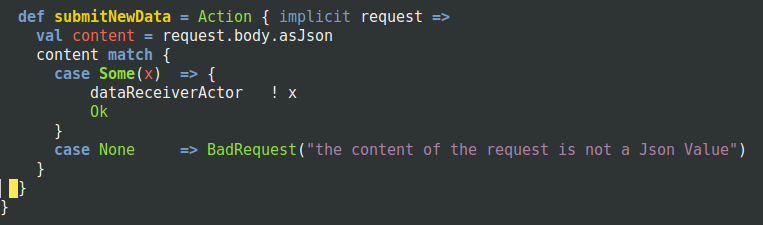
\includegraphics[scale=0.5,natwidth=610,natheight=642]{Figures/Project/Server/Interaction/SaveDataStream/DataStream1.png}
\caption{Step 1 - Stream di Salvataggio D@ati}
\label{SaveDataStream1}
\end{figure}

\begin{figure}[h]
\centering
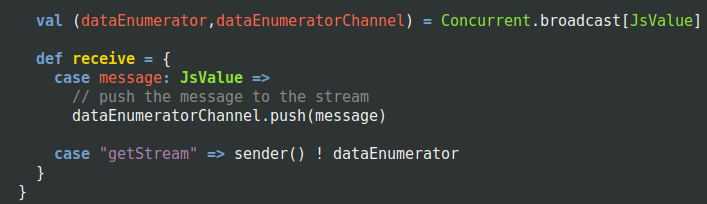
\includegraphics[scale=0.5,natwidth=610,natheight=642]{Figures/Project/Server/Interaction/SaveDataStream/DataStream2.png}
\caption{Step 2 - Stream di Salvataggio Dati}
\label{SaveDataStream2}
\end{figure}

\begin{figure}[h]
\centering
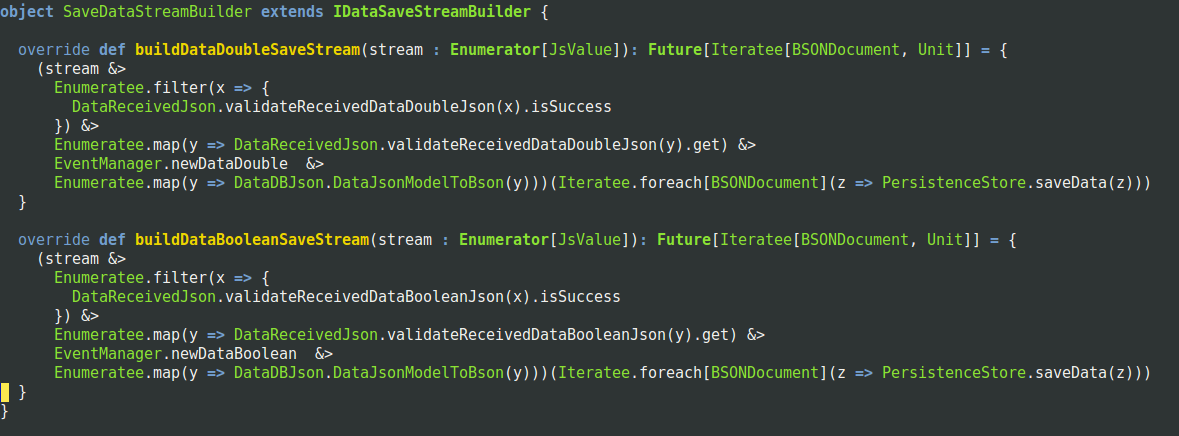
\includegraphics[scale=0.3,natwidth=610,natheight=642]{Figures/Project/Server/Interaction/SaveDataStream/DataStream3.png}
\caption{Step 3 - Stream di Salvataggio Dati}
\label{SaveDataStream3}
\end{figure}

\begin{figure}[h]
\centering
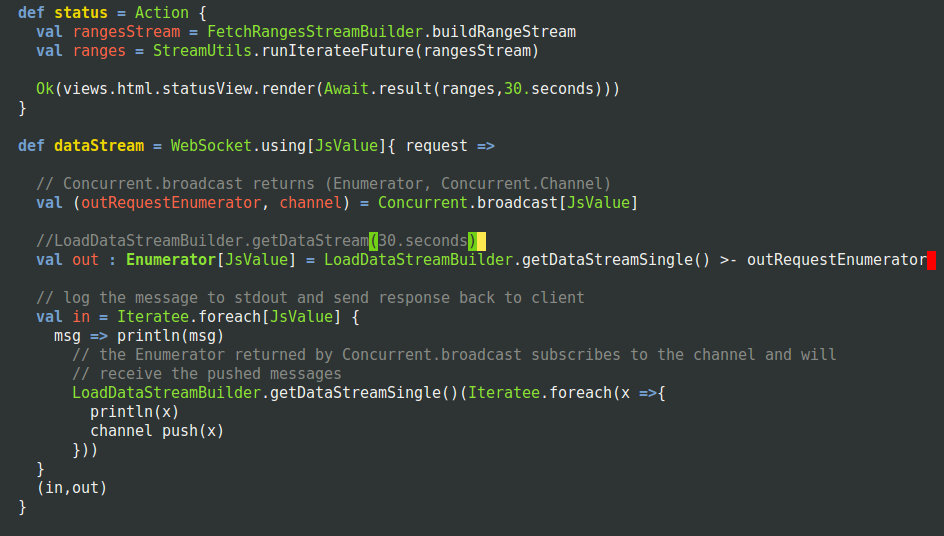
\includegraphics[scale=0.3,natwidth=610,natheight=642]{Figures/Project/Server/Interaction/LoadDataStream/LoadDataStream1.png}
\caption{Step 1 - Stream di Caricamento Dati}
\label{LoadDataStream1}
\end{figure}

\begin{figure}[h]
\centering
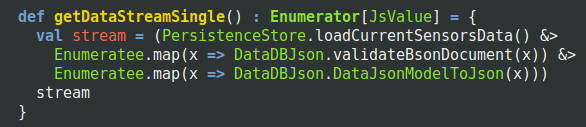
\includegraphics[scale=0.5,natwidth=610,natheight=642]{Figures/Project/Server/Interaction/LoadDataStream/LoadDataStream2.png}
\caption{Step 2 - Stream di Caricamento Dati}
\label{LoadDataStream2}
\end{figure}

\begin{figure}[h]
\centering
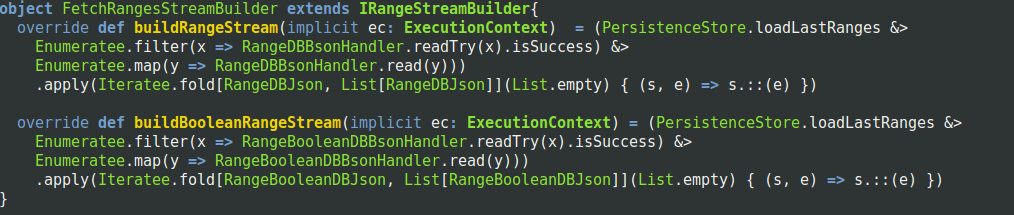
\includegraphics[scale=0.3,natwidth=610,natheight=642]{Figures/Project/Server/Interaction/RangeLoadStream/RangeLoadStream.png}
\caption{Stream di Caricamento Ranges}
\label{LoadRangeStream}
\end{figure}

\begin{figure}[h]
\centering
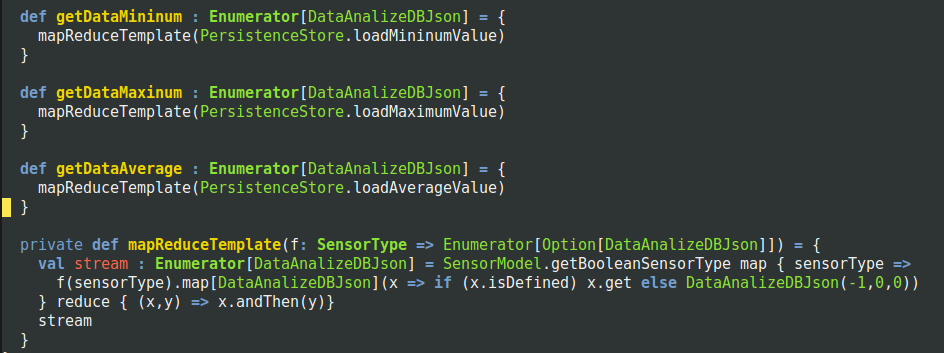
\includegraphics[scale=0.3,natwidth=610,natheight=642]{Figures/Project/Server/Interaction/AnalysisLoadStream/AnalysisLoadStream.png}
\caption{Stream di Caricamento Dati di Analysis}
\label{AnalysisRangeStream}
\end{figure}


\afterpage{\clearpage}

\newpage

\subsection{Comportamento}

Per quanto concerne il comportamento, verranno mostrati gli stati attraverso i quali il server transita durante il suo funzionamento. Avendo utilizzato un approccio reactive e funzionale dove possibile, il numero di stati collezionati all'interno delle varie entit\`a si riduce. Infatti si \`e cercato di utilizzare tipi \textit{object} dove possibile, che corrispondono a un singleton pattern, ma solamente che istanziati da parte del framework. In particolare questi oggetti non contengono dello stato.\\
Solo la classe \textit{RangeChecker} contiene uno stato che corrisponde alla collezione dei range attualmente attivi all'interno del server. Le uniche altre classi che si sono implementate sono quelle che effettivamente costituiscono l'oggetto \textit{PersistenceStore} secondo uno strategy pattern. Si \`e scelto di lasciarle come classi in quanto possano essere dinamicamente interscambiabili con altri oggetti che possono operare su basi di dati differenti, ma mantenendo lo stesso contratto/interfaccia.\\
Per quanto concerne la lista di stati necessari tutto si riduce a:
\begin{enumerate}
\item \textbf{Inizializzazione:} eseguita maggiormente dal sistema che si occupa di creare gli object e quindi instanziare tutte le loro dipendenze in base a quello che viene definito nei loro costruttori. Questa operazione viene effettuata in maniera lazy in modo da enfatizzare la velocit\`a di esecuzione e ridurre l'utilizzo di risorse inutili al momento.
  \item \textbf{Modifica dei Range:} Alla modifica dei range deve conseguire anche una modifica in memoria della collection che contiene i range attivi al momento, quindi si attiva un processo di aggiornamento nell'oggetto \textit{RangeChecker}. Quando questo processo termina il suo decorso il tutto torna a funzionare sulla base della costruzione degli stream che si \`e discussa in  fase di analisi.
\end{enumerate}

Per quanto riguarda lo schema del comportamento quindi tutto diventa semplicemente:

\begin{figure}[h]
\centering
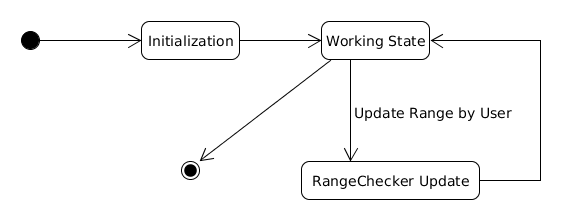
\includegraphics[scale=0.5,natwidth=610,natheight=642]{Figures/Project/Server/Behaviour/DomoticRoomServerStateDiagram.png}
\caption{Schema di Behaviour del server}
\label{BehaviourServerSchema}
\end{figure}

\newpage

\begin{center}
  \textbf{Sistema Embedded}
\end{center}

\subsection{Struttura}
La struttura del Sistema Embedded non ha subito cambiamenti drastici dalla progettazione logica, sono state solo apportate alcune modifiche necessarie per i limiti e le propriet\`a imposte dall Hardware e dalle tecnologie utilizzate.
La prima modifica è l'assenza delle Interface, sostituite interamente dalle classi Abstract, questo perch\'e Python non prevede l'implementazione delle Interface.
L'entit\`a \textit{ASensor} quindi rappresenta il comportamento comune a tutti i sensori, come l'inizializzazione sulla GPIO Board.
La classe ASensor poi viene effettivamente implementata dalle classi:
\begin{itemize}
\item \textit{TemperatureSensor}: Rappresenta il sensore di Temperatura, il quale dopo un intervallo di tempo determinato all'istanzazione richiede al sensore il valore percepito.
\item \textit{BooleanSensor}: I sensori Booleani invece comunicano col Sistema in modo Asincrono notificando solamente quando percepiscono un cambiamento dell'ambiente monitorato.
\end{itemize}

Si pu\`o quindi notare come il sensore di temperatura sia gestito a polling dal sistema, con letture fatte ad intervalli regolari; a differenza dei sensori Booleani che invece vengono gestiti tramite Interupt.

Ogni sensore implementa un canale Stream per l'invio dei dati, come previsto dal progetto logico.
I dati inviati nel canale Stream vengono elaborati dalle entità di tipo AStreamWorker, le quali vengono poi implementate in differenti specializzazioni, in base al compito a loro affidato:
\begin{itemize}
\item \textit{Validator}: Il Validator \`e l'unica entit\`a dal prevista inizialmente dal progetto logico, \`e stata aggiunta perch\'e si occupa di validare tramite checksum il valore ricevuto dal sensore di Temperatura.
\item \textit{Converter}: Il Converter invece modifica i valori ricevuti dal Validator secondo una particolare funzione di conversione.
\item \textit{Packager}: Il Packager trasforma i dati ricevuti dai Convert in una stringa in formato Json che contiene tutte le informazioni necessarie al Server.
\item \textit{Sender}: L'ultimo StreamWorker \`e rappresentato dal Sender che invia la stringa Json tramite richiesta http al Server.
\end{itemize}

Infine \`e stata implementata \textit{DomoticRoomBuilder} per l'inizializzazione del Sistema Embedded, la quale inizializza i Sensori e il reticolo di StreamWorker necessario per la gestione dei valori.

\subsection{Interazione}

\begin{figure}[ht]
\centering
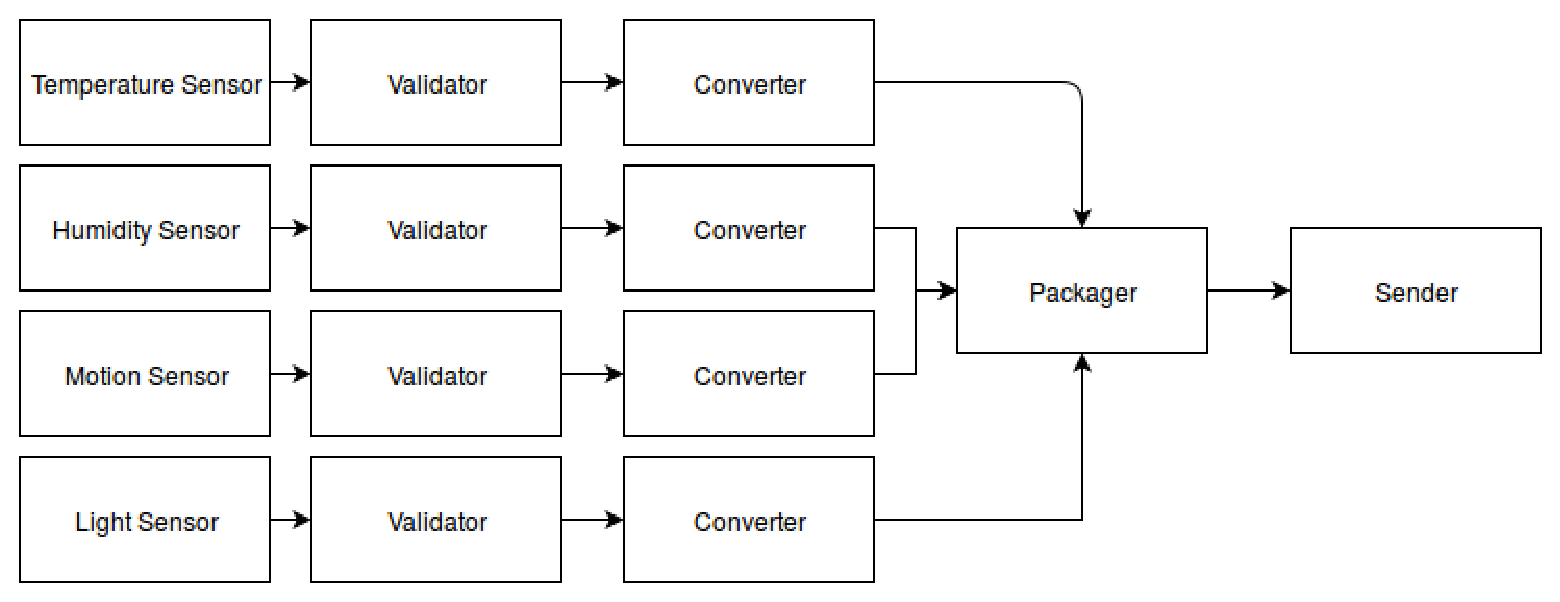
\includegraphics[scale=0.5]{Figures/Project/EmbeddedSystem/FlowDiagram1}
\caption{Marable diagram dei singoli dati proveniente da una sorgente}
\end{figure}

L'interazione del sistema Embedded è rimasta pressoch\'e invariata da quanto descritto nel progetto logico.
L'introduzione dell'entit\`a Validator aggiunge, semplicemente, un altro passaggio al flusso di elaborazione dei dati rilevati dai sensori.
Questo dimostra come il flusso di StreamWorker sia una struttura molto flessibile ed estendibile in base alle necessità del sistema.

\subsection{Comportamento}

Il sistema viene inizializzato dalla classe \textit{DomoticRoomBuilder}, la quale inizializza i sensori e crea gli StreamWorker necessari alla gestione del flusso dei dati.
L'unica informazione richiesta all'utente è l'indirizzo IP e la porta tramite cui comunicare col Server.
